\documentclass[review]{elsarticle}
\usepackage{amsthm, amsmath, amsfonts, amssymb}
\usepackage{lineno,hyperref}
\usepackage{graphicx}
\usepackage{url}
\usepackage[nolists,nomarkers]{endfloat}
\usepackage{setspace}
\doublespacing

\modulolinenumbers[5]
\journal{Journal of Biomechanics}
\bibliographystyle{model4-names}

\begin{document}
\begin{frontmatter}
\title{Dissipative particle dynamics simulation of cell entry into a micro-channel}

\author[zhou]{Lvwen Zhou}
\address[zhou]{Institute of Mechanics, Chinese Academy of Sciences, Beijing 100190, China}

\author[Zhang]{Yuqian Zhang}
\address[Zhang]{Cancer Institute \& Hostptial, Chinese Academy of Medical Sciences, Beijing 100021, China}

\author[Deng]{Xiaolong Deng}
\address[Deng]{Beijing Computational Science Research Center, Beijing 100084, China}

\author[Liu]{Moubin Liu\corref{mycorrespondingauthor}}
\address[Liu]{College of Engineering, Peking University, Beijing 100871, China}
\cortext[mycorrespondingauthor]{Corresponding author}
\ead{mbliu@pku.edu.cn}

%%%%%%%%%%%%%%%%%%%%%%%%%%%%%%%%%%%%%%%%%%%%%%%%%%%%%%%%%%%%%%%%%%%%%%%%%%%%%%
\begin{abstract}
Cell deformability is an important biomarker which can be used to distinguish and sort between healthy and cancer cells. In this paper, we presented a dissipative particle dynamics (DPD) model for investigating cell entry into micro-channels. The cell membrane is represented by a network of DPD particles (beads) connected by worm-like chain (WLC) springs, which is able to mimic the viscoelastic effect of the membrane.  The entry process of benign breast epithelial cells (MCF-10A) and non-metastatic tumor breast cells (MCF-7) through a constricted micro-channel are comparatively investigated using this DPD model.  It is shown that both the time histories of the cell displacement and the dynamic behaviors of cell entry agree with experimental observations. The entry time of MCF-10A cell is approximately four times of that of MCF-7 cell since MCF-10A cells are stiffer than MCF-7 cells.  It is demonstrated that the presented DPD method is effective in modeling cell deformability, and the obtained results can be helpful in understanding how cells with different mechanical properties respond to physical loads.
\end{abstract}

\begin{keyword}
Cell entry\sep Micro-channel \sep Dissipative particle dynamics (DPD)
\MSC[2010] 00-01\sep  99-00
\end{keyword}

\end{frontmatter}

\linenumbers

%%%%%%%%%%%%%%%%%%%%%%%%%%%%%%%%%%%%%%%%%%%%%%%%%%%%%%%%%%%%%%%%%%%%%%%%%%%%%%
\section{Introduction}
Dynamical behaviors of migration and deformation variations of cells in confined environment are probably caused by pathological changes in mechanical properties of cells, which may be closely related to several cell diseases. These variations are often facilitated by the altering in the mechanical behaviors of cells such as large changes of elastic modulus \cite{hosseini_particle-based_2009}. Modern physiology and medicine have established the relationship of mechanical variations between healthy and pathological cells. For example, compared to healthy cells, diseased cells such as cancer cells are known to have different stiffness and elasticity \cite{lee_biomechanics_2007}. Such differences can be used to distinguish between normal and diseased cells \cite{bathe_neutrophil_2002,hou_deformability_2009}. Recently, increased micro-fluidic devices were designed and applied in medical diagnostics to diagnose and treat cells disease \cite{suresh_biomechanics_2007,liu_microfluidic_2010}. 
Thus, investigating cell entry into micro channels can be fundamentally important and it is of significance to understand how cells with different mechanical properties respond to physical loads, and to further design more effective micro-fluidic devices. 

In this work, we present a DPD model for simulating the entry process of  MCF-10A and MCF-7 cells through a constricted micro-channel. Cell model is described in section \ref{cell}.  Numerical simulations of MCF-10A and MCF-7 cells through a constricted micro-channel are presented and analyzed in section \ref{simulation} and \ref{results}. The paper concludes in section \ref{conclusion} with some remarks. 
%%%%%%%%%%%%%%%%%%%%%%%%%%%%%%%%%%%%%%%%%%%%%%%%%%%%%%%%%%%%%%%%%%%%%%%%%%%%%%
\section{Methods}\label{cell}

\subsection{DPD method}
Dissipative particle dynamics (DPD) \cite{hoogerbrugge_simulating_1992} is a mesoscopic method which describes clusters of molecules (particle) moving together in a Lagrangian fashion subject to soft quadratic potentials. The total force acting on a DPD particle $i$ is given by a sum over all particles $j$ that lie within a fixed cut-off distance, of three pairwise-additive forces:
\begin{equation}\label{Forcesum}
\mathbf{f}_{i}  = \sum_{j\neq i} \mathbf{F}_{ij}^\mathrm{C} + \mathbf{F}_{ij}^\mathrm{D} + \mathbf{F}_{ij}^\mathrm{R}
\end{equation}
where $\mathbf{F}_{ij}^\mathrm{C}$ is a conservative force, $\mathbf{F}_{ij}^\mathrm{D}$ and $\mathbf{F}_{ij}^\mathrm{R}$ is a dissipative force and a random force. The conservative force acts to give particle a chemical identity, while the dissipative and random forces together form a thermostat that keeps the mean temperature of the system constant. For more detailed information about methodology and applications of DPD, see references \cite{hoogerbrugge_simulating_1992,liu_dissipative_2014}.

\subsection{Cell membrane model}
In this section, we construct cell membrane model using DPD. There are four types of particles in our DPD system,  as shown in figure \ref{fig:4particles}. 
\begin{figure}[!htb]
\centering
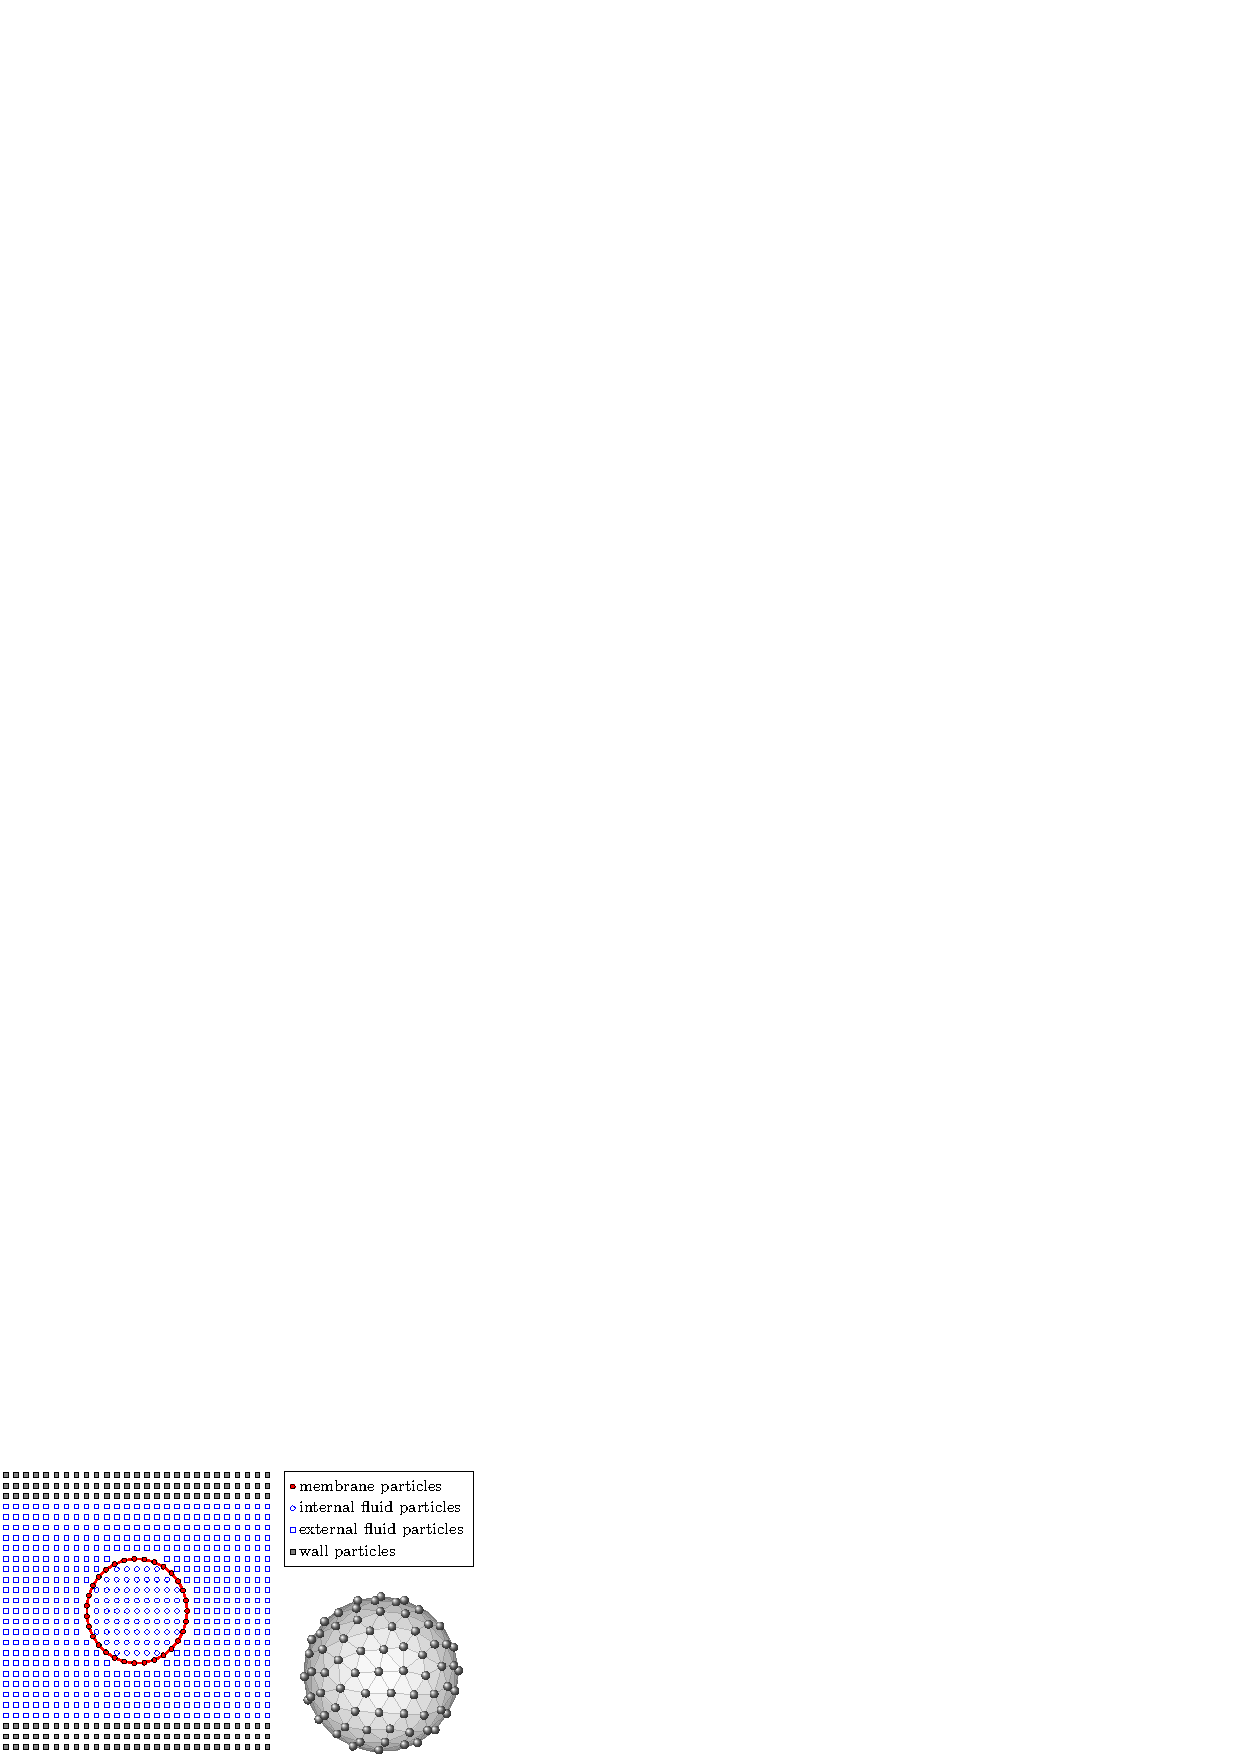
\includegraphics{4typeparticles.pdf}
\caption{DPD system with four types of particles. Cell membrane model represented by a network of springs linked DPD particles.}\label{fig:4particles}
\end{figure}
The cell membrane structure is defined by a two-dimensional triangular network on the spherical surface. Each link of triangular network is modelled by nonlinear WLC spring model \cite{marko_stretching_1995}. The force between membrane particles includes the elastic and viscous parts. The elastic part is characterized by an energy potential, given by
\begin{equation}\label{eq:free_energy}
\mathbf{f}_i^\textrm{elastic} = \frac{\partial U(\{\mathbf{r}_i\})}{\partial \mathbf{r}_i}, \quad U(\{\mathbf{r}_i\}) = U_{\textrm{in-plane}} + U_{\mathrm{bending}} + U_{\mathrm{volume}}
\end{equation}

\section{Simulation}\label{simulation}
In Hou et al.'s study \cite{hou_deformability_2009}, a microfabricated fluidic channel design consisting of a straight channel and two reservoirs, as shown in figure \ref{fig:experimental_setup}, was used to study the biorheological behaviour of MCF-10A cells and MCF-7 cells to develop a method to distinguish between non-malignant and malignant cells. 
The fluidic channel is 150 $\mu m$ in length and has a square cross section area of 10 by 10 $\mu m$ with a 45$^\circ$ tapered entrance. Flow in the micro-channel is driven by a differential pressure $\Delta p = 490.5 \mathrm{Pa}$ established between both ends of the setup. Under experimental conditions at room temperature of $22-24 ^\circ\mathrm{C}$, the cells have to deform to pass through the channel, allowing quantification of several physical parameters such as entry time, transit velocity and elongation index. 
\begin{figure}[!htb]
\centering
%\tikzfigure{3Dchannel.tikz}
\includegraphics{3Dchannel.pdf}
\caption{\label{fig:experimental_setup}Schematic of a micro-channel with a tapered entrance}
\end{figure}


%%%%%%%%%%%%%%%%%%%%%%%%%%%%%%%%%%%%%%%%%%%%%%%%%%%%%%%%%%%%%%%%%%%%%%%%%%%%%%
\section{Results}\label{results}
In this section, MCF-10A cell is firstly studied by DPD simulating and compared with the experiment, and then MCF-7 cell is also studied and compared with simulation results of MCF-10A cell. 

\subsection{MCF-10A passing through a confined micro-channel}
In DPD simulation, the cell is initially positioned at a distance of 25 from the channel entrance to give the cell initial transient period to reach steady velocity before entry. Figure \ref{fig:Snapshots-DPD} shows snapshots of MCF-10A cell through the micro-channel.
\begin{figure}[!htb]
\centering
%\tikzfigure{Snapshots-DPD.tikz}
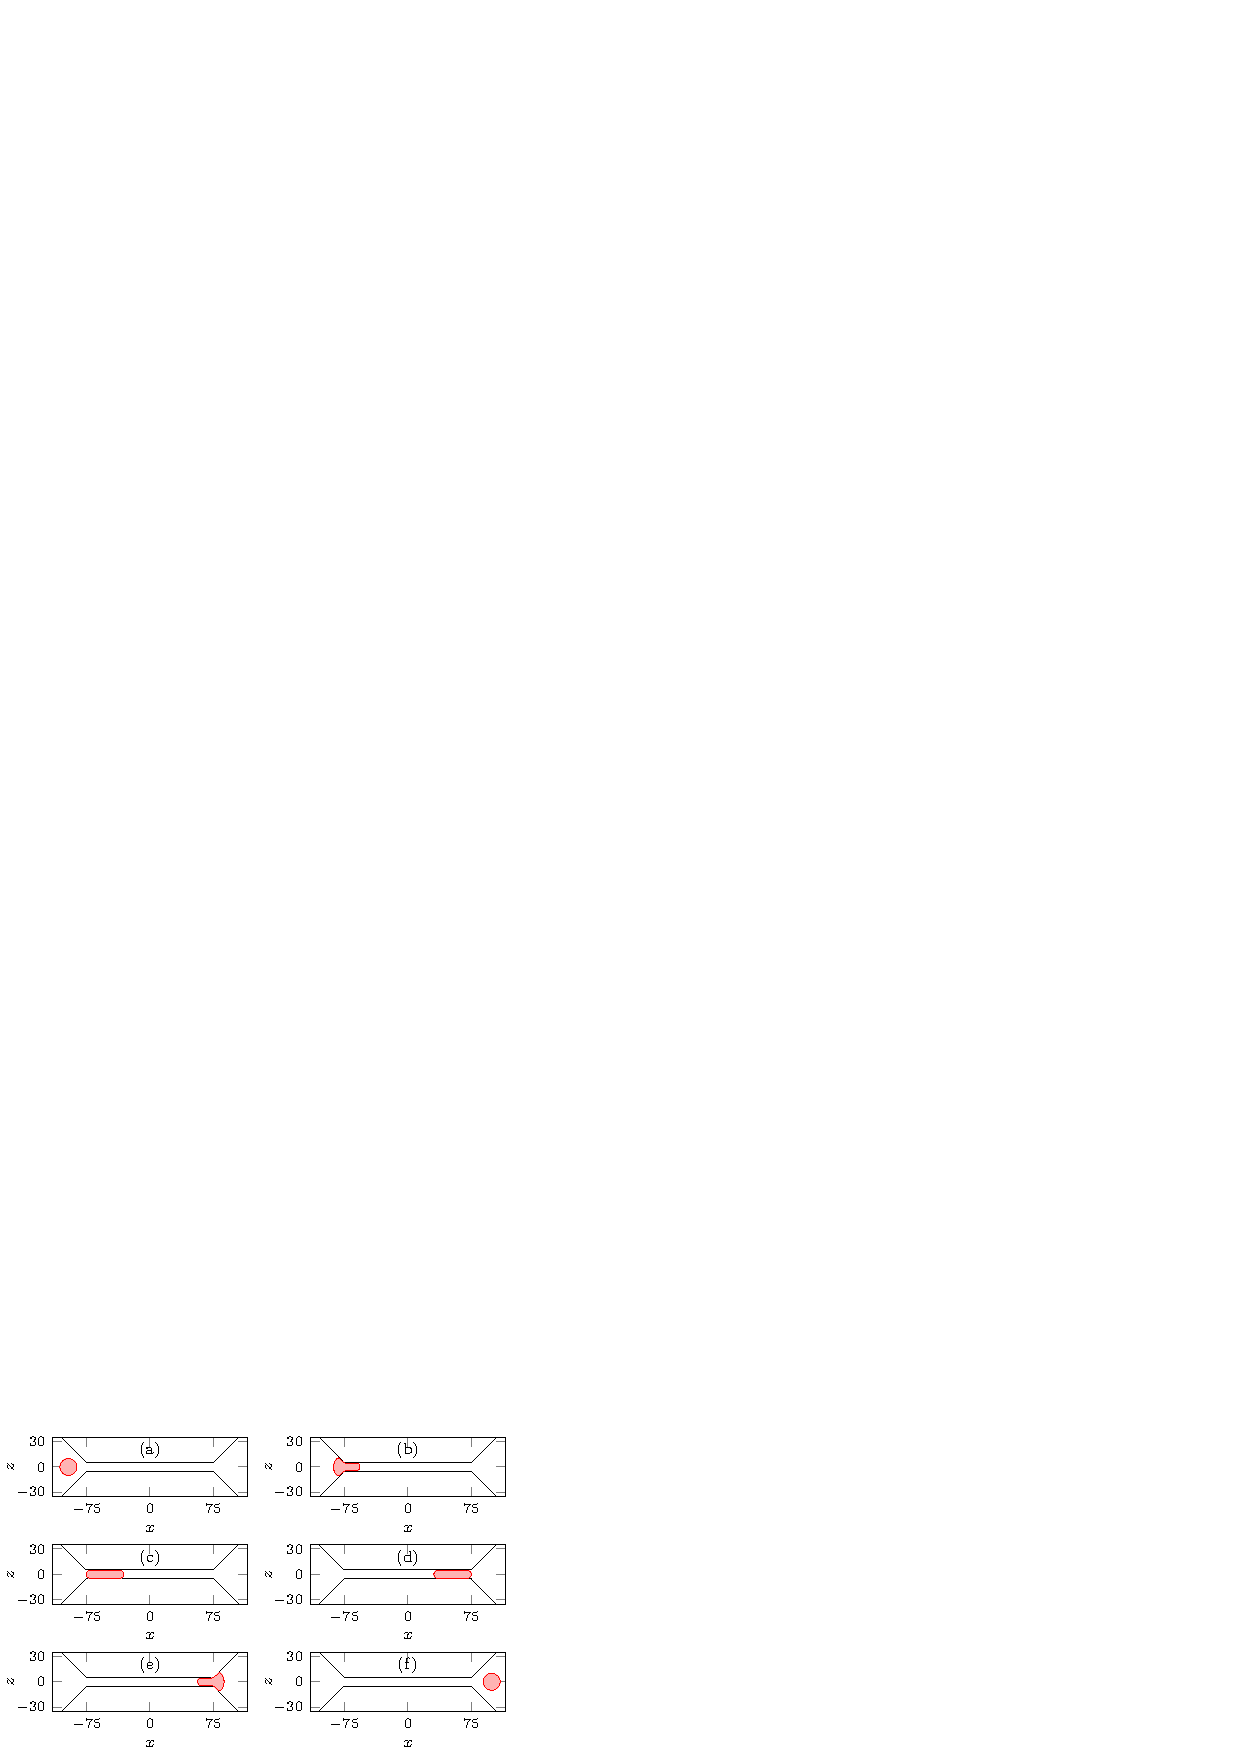
\includegraphics{Snapshots-DPD.pdf}
\caption{Snapshots of MCF-10A cell traversing across a micro-channel from DPD simulation.} \label{fig:Snapshots-DPD}
\end{figure}

%%%%%%%%%%%%%%%%%%%%%%%%%%%%%%%%%%%%%%%%%%%%%%%%%%%%%%%%%%%%%%%%%%%%%%%%%%%%%%
\section{Conclusion}\label{conclusion}

This paper presented a DPD model for simulating the movement and deformability of single cells when entering micro-channels with confined structures.  The entry processes of MCF-10A and MCF-7 cells are comparatively investigated. We conclude that the presented DPD method with WLC spring to model cells is effective in simulating cell entry into micro-channels. Both the cell displacement time-plots and the dynamical behavior of the cell entry are shown to match quantitatively throughout the cell entry, subjected to experimental uncertainties and model assumptions. Furthermore, the model allowed us to confirm that MCF-10A cells have longer entry time than MCF-7 cells of similar sizes because MCF-10A cells are stiffer than MCF-7 cells. These quantitative agreements show the usefulness and effectiveness of our models in interpreting cellular experiments.

%%%%%%%%%%%%%%%%%%%%%%%%%%%%%%%%%%%%%%%%%%%%%%%%%%%%%%%%%%%%%%%%%%%%%%%%%%%%%%
\section*{Conflict of interest statement}
All authors disclose that there was no conflict of interest regarding this work.
\section*{Acknowledgement}
This work has been supported by the National Natural Science Foundation of China (31370953 \& 10942004).

\section*{References}
\bibliography{main}
\end{document}
